\section{PuzzleJAX}

\section{Boxoban}

\section{Agent Architecture}
To create an agent that can plan ahead in the sparse reward landscape, we will use an AlphaGo-style agent where a treesearch is driven by a policy function $\pi$ and a value function $V$ that takes in the current puzzle state $s_t$ preprocessed by some compression function $c$. The policy function outputs an action logit $a$ that the treesearch prioritizes for searching and the value function outputs a scalar value that determines the 'usefulness' of the input state. 

$$a_t = \pi_\theta(c(s_t))$$

$$v_t = V_\phi(c(s_t))$$

In order to solve Sokoban puzzles, one must first understand the dataset. The dataset is Boxoban, a set of 9 million Sokoban puzzles in a 10x10 2d space. These levels can be used to yield solution trajectories using Breath First Search. The BFS search outputs pairs of puzzle state and correct actions. The idea is to pretrain the policy network and the value network using this solution BFS trajectory and finetune the value network with reinforcement learning in order to create an agent that can solve unseen sokoban levels more efficiently compared to MCTS or BFS.

Principle Component Analysis can reveal characteristics of values against each other. By performing Multilinear Principle Component Analysis on the solution trajectories, we can discover interesting features of the trajectories.

\begin{figure}[!ht] % [h] forces the image to be placed "here"
    \centering
    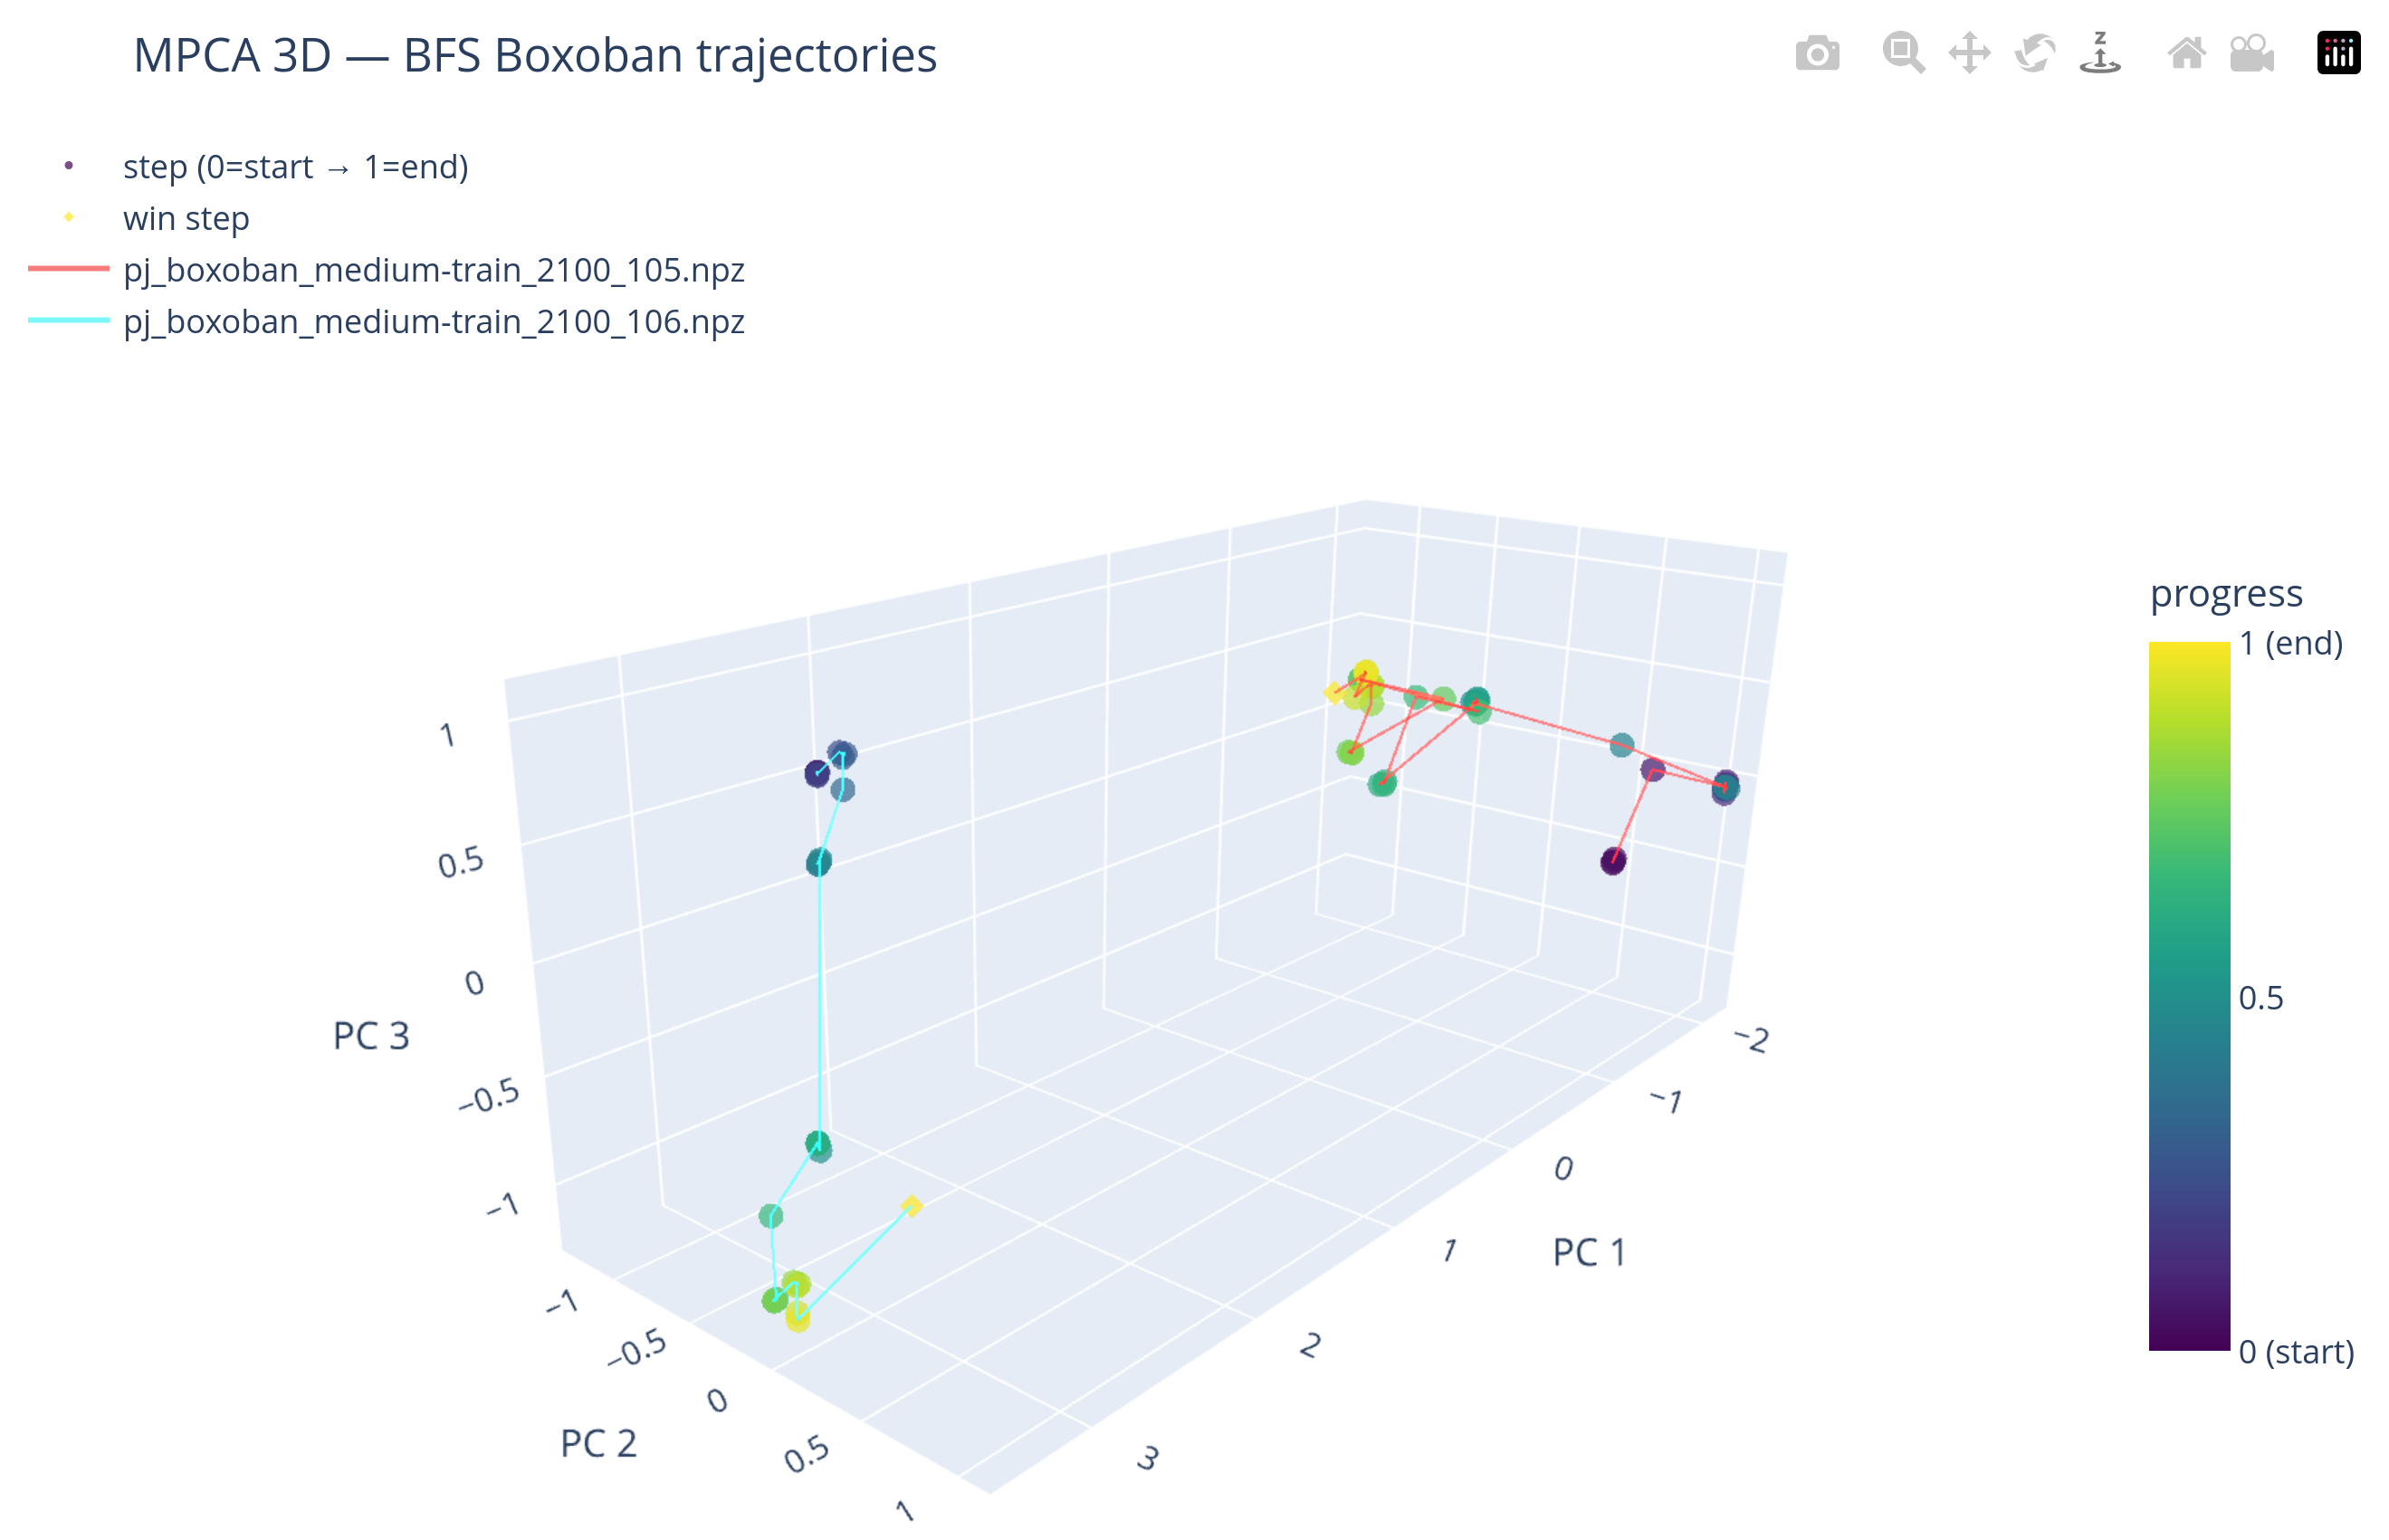
\includegraphics[width=1\textwidth]{images/mpca_less.png} 
    \caption{MPCA visualization of a Boxoban solution trajectory. Each point represents a state $s_t$, with colors transitioning from start (dark) to finish (yellow). The curvilinear relationship demonstrates that states are sequentially dependent; this inherent temporal structure justifies the use of recurrent architectures (RNNs) or Transformers, which utilize a hidden state $h_{t-1}$ to provide the necessary contextual memory for accurate action prediction.}
    \label{fig:mpca_less}
\end{figure}

First, the graph reveals that solution steps of the same puzzle are more closely related to each other than to other puzzles. This may seem obvious due to the trajectories maintaining distinct wall structure through its multihot layers, however this becomes more relevant when considering another discovery.

More importantly, most trajectories form a curve in the PCA space. With the starting state and the ending state being furthest in most puzzles, the trajectories form a curve. This is true when plotting a trajectory of a single level. This signifies that it is possible to predict the puzzle solution trajectory on the PCA space by fitting on the trajectory.

Since each trajectories are uniquely apart from each other while displaying strong curvilinear relation, one can conclude that the contextual data is critical for successfully predicting the solution move. This prompts the value function to become self-dependent to its previous state to have the memory capacity. This can be done in several methods such as using recurrent neural network or transformers. The value function can then be defined as follows.


$$a_t, h_t = \pi_\theta(c(s_t) | h_{t-1})$$

$$v_t, h_t = V_\phi(c(s_t) | h_{t-1})$$

\section{Input Compression Stategies}

\subsection{CNN}

\subsection{Autoencoder}

\subsection{DCT}

\section{Agent Architecture}

\subsection{Policy Network}

\subsection{Value Network}

